\documentclass[dvisvgm,border=0pt]{standalone}
\usepackage[T1]{fontenc}
\usepackage{newtxtext,newtxmath}
\usepackage{tikz}
\usetikzlibrary{arrows.meta,decorations.pathmorphing}

\definecolor{Navy}{HTML}{08154F}
\definecolor{Ink}{HTML}{2B5098}
\definecolor{Blue}{HTML}{315EDB}
\definecolor{BlueTint}{HTML}{DCEBFC}
\definecolor{Sage}{HTML}{568638}
\definecolor{SageTint}{HTML}{E7F2E1}
\definecolor{Gold}{HTML}{F3B122}
\definecolor{Ice}{HTML}{F3FAFF}
\definecolor{Rule}{HTML}{CAE1FA}
\definecolor{Muted}{HTML}{8B95AA}

\tikzset{
  state/.style={draw=Blue,fill=BlueTint,line width=3bp,rounded corners=10bp},
  operation/.style={draw=Sage,fill=SageTint,line width=3bp,rounded corners=10bp},
  wire/.style={draw=Blue,line width=3bp,line cap=round,line join=round},
  blue arrow/.style={wire,-{Stealth[length=13bp,width=12bp]}},
  gold arrow/.style={draw=Gold,line width=6bp,line cap=round,-{Stealth[length=19bp,width=20bp]}},
  time arrow/.style={draw=Muted,line width=3bp,-{Stealth[length=17bp,width=15bp]}},
}

\newcommand{\figbackground}[2]{
  \path[use as bounding box] (0,0) rectangle (#1,#2);
  \fill[Ice!45] (0,0) rectangle (#1,#2);
}

\newcommand{\figtext}[5][Navy]{
  \node[text=#1,font=\fontsize{#4}{#4}\selectfont,inner sep=0bp,align=center]
    at (#2,#3) {#5};
}

\newcommand{\figmath}[5][Navy]{
  \figtext[#1]{#2}{#3}{#4}{$\displaystyle #5$}
}

\newcommand{\panelheading}[3]{
  \fill[BlueTint] (#1,190) circle (35bp);
  \node[text=Navy,font=\fontsize{40}{42}\selectfont\bfseries,inner sep=0bp]
    at (#1,190) {#2};
  \node[text=Navy,anchor=west,font=\fontsize{40}{42}\selectfont\bfseries,inner sep=0bp]
    at ({#1+62},190) {#3};
}

\newcommand{\panelrules}{
  \draw[Rule,line width=2bp] (535,162) -- (535,733);
  \draw[Rule,line width=2bp] (1090,162) -- (1090,733);
}

\newcommand{\statebox}[4]{
  \fill[Blue,opacity=.08,rounded corners=10bp]
    ({#1+4},{#2+6}) rectangle ({#3+4},{#4+6});
  \draw[state] (#1,#2) rectangle (#3,#4);
}

\newcommand{\operationbox}[4]{
  \fill[Sage,opacity=.08,rounded corners=10bp]
    ({#1+4},{#2+6}) rectangle ({#3+4},{#4+6});
  \draw[operation] (#1,#2) rectangle (#3,#4);
}

\newcommand{\processstrip}[4]{
  \fill[BlueTint!70,rounded corners=20bp] (50,762) rectangle (1622,858);
  \foreach \x/\word in {132/#1,522/#2,912/#3,1302/#4} {
    \fill[BlueTint,rounded corners=15bp] (\x,781) rectangle ({\x+306},837);
    \node[text=Navy,font=\fontsize{30}{34}\selectfont\bfseries,inner sep=0bp]
      at ({\x+153},809) {\word};
  }
  \foreach \x in {465,855,1245} {
    \draw[gold arrow] (\x,809) -- ({\x+31},809);
  }
}


\begin{document}
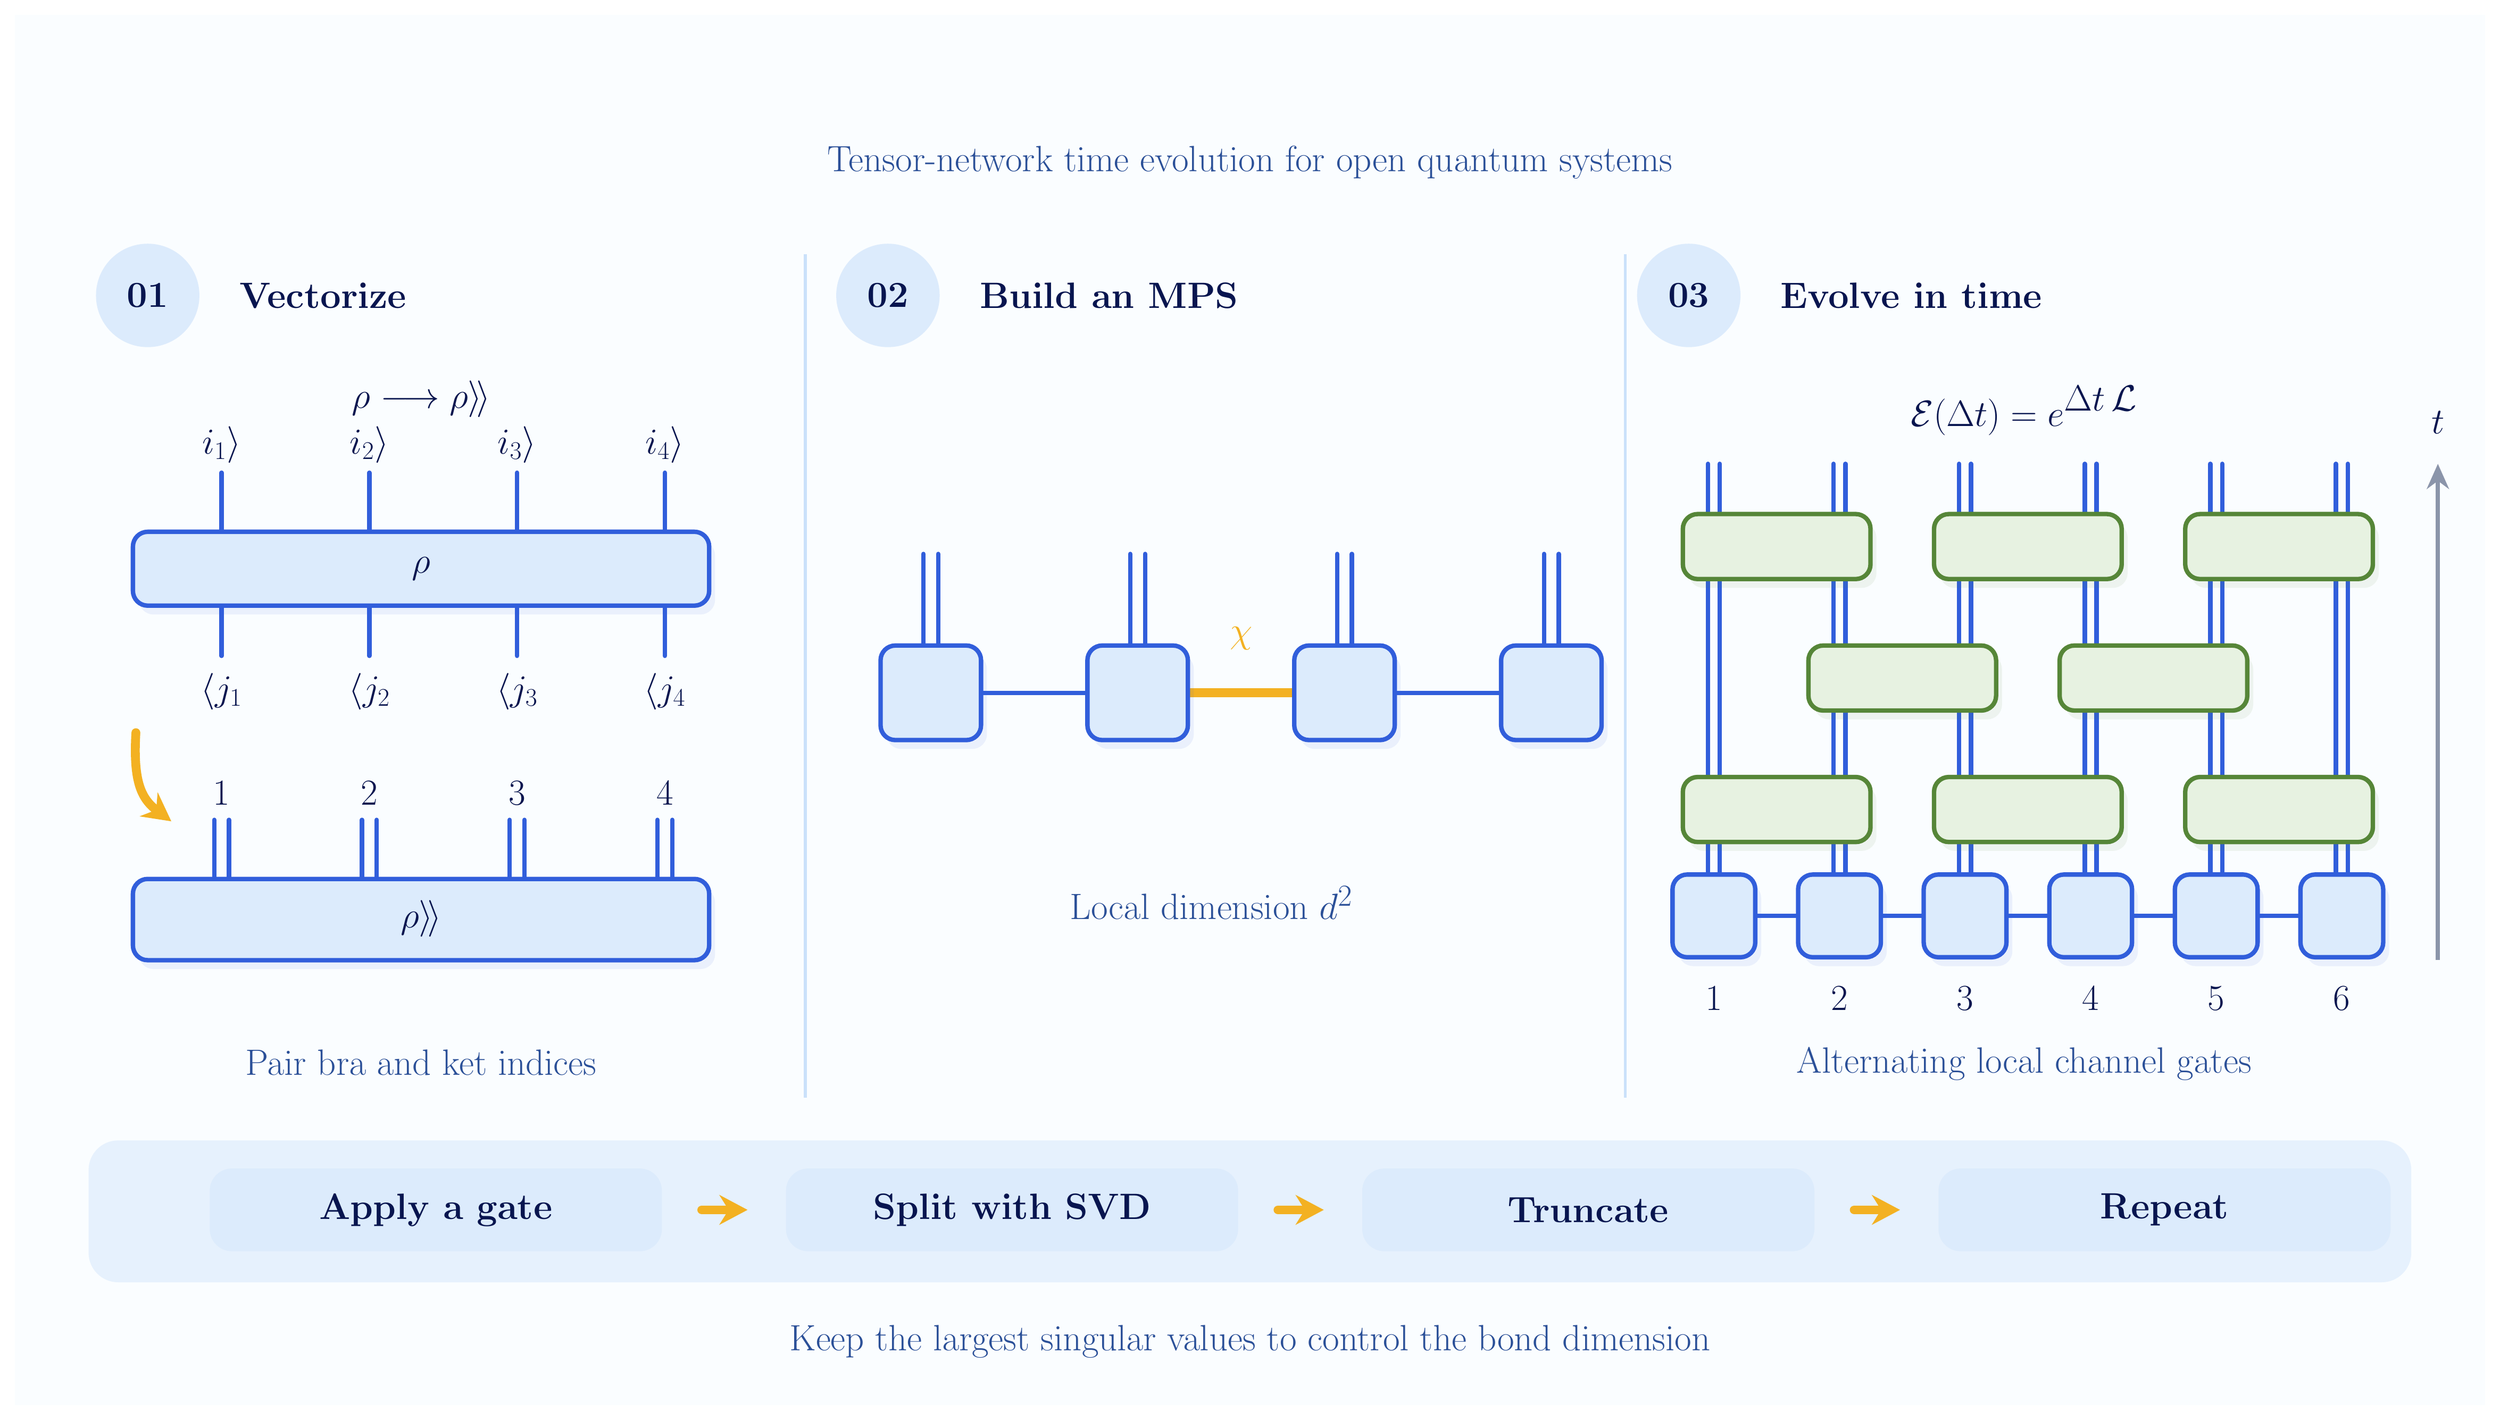
\begin{tikzpicture}[x=1bp,y=-1bp]
  \figbackground{1672}{941}
  \figtext[Ink]{836}{100}{38}{Tensor-network time evolution for open quantum systems}
  \panelrules
  \panelheading{90}{01}{Vectorize}
  \panelheading{591}{02}{Build an MPS}
  \panelheading{1133}{03}{Evolve in time}

  % Density operator: separate ket and bra indices at each site.
  \figmath{275}{260}{39}{\rho \longrightarrow \lvert\rho\rangle\!\rangle}
  \foreach \x/\i in {140/1,240/2,340/3,440/4} {
    \draw[wire] (\x,310) -- (\x,350);
    \draw[wire] (\x,400) -- (\x,434);
    \figmath{\x}{291}{25}{\lvert i_{\i}\rangle}
    \figmath{\x}{458}{25}{\langle j_{\i}\rvert}
  }
  \statebox{80}{350}{470}{400}
  \figmath{275}{375}{37}{\rho}
  \draw[gold arrow] (82,486) .. controls (80,520) and (86,531) .. (106,546);
  \foreach \x/\i in {140/1,240/2,340/3,440/4} {
    \draw[wire] ({\x-5},545) -- ({\x-5},585);
    \draw[wire] ({\x+5},545) -- ({\x+5},585);
    \figtext{\x}{527}{25}{\i}
  }
  \statebox{80}{585}{470}{640}
  \figmath{275}{612}{38}{\lvert\rho\rangle\!\rangle}
  \figtext[Ink]{275}{709}{31}{Pair bra and ket indices}

  % Matrix product state with paired physical legs and horizontal bonds.
  \draw[wire] (620,459) -- (1040,459);
  \draw[Gold,line width=6bp] (794,459) -- (866,459);
  \foreach \x in {620,760,900,1040} {
    \draw[wire] ({\x-5},365) -- ({\x-5},427);
    \draw[wire] ({\x+5},365) -- ({\x+5},427);
    \statebox{\x-34}{427}{\x+34}{491}
  }
  \figmath[Gold]{830}{422}{38}{\chi}
  \figtext[Ink]{810}{601}{32}{Local dimension $d^2$}

  % Six fused bra-ket site wires; the layers act on (12,34,56)/(23,45).
  \foreach \x in {1150,1235,1320,1405,1490,1575} {
    \draw[wire] ({\x-4},304) -- ({\x-4},582);
    \draw[wire] ({\x+4},304) -- ({\x+4},582);
  }
  \foreach \x in {1150,1320,1490} {
    \operationbox{\x-21}{338}{\x+106}{382}
    \operationbox{\x-21}{516}{\x+106}{560}
  }
  \foreach \x in {1235,1405} {
    \operationbox{\x-21}{427}{\x+106}{471}
  }
  \draw[wire] (1150,610) -- (1575,610);
  \foreach \x/\i in {1150/1,1235/2,1320/3,1405/4,1490/5,1575/6} {
    \statebox{\x-28}{582}{\x+28}{638}
    \figtext{\x}{666}{25}{\i}
  }
  \draw[time arrow] (1640,640) -- (1640,304);
  \figmath{1640}{276}{35}{t}
  \figmath{1360}{268}{37}{\mathcal{E}(\Delta t)=e^{\Delta t\,\mathcal{L}}}
  \figtext[Ink]{1360}{710}{29}{Alternating local channel gates}

  \processstrip{Apply a gate}{Split with SVD}{Truncate}{Repeat}
  \figtext[Ink]{836}{898}{28}{Keep the largest singular values to control the bond dimension}
\end{tikzpicture}
\end{document}
